\ExplSyntaxOn
\int_gset:Nn \g__ptxcd_interlude_page_int {-1}
\ExplSyntaxOff

\interlude{What do we want?}

\begin{frame}[T]{}
  \centering
  \bsixonetwo

  { \footnotesize What do we want? }
  \\[-0.00cm] \resizebox{10cm}{!}{\bfseries \Large data communication}
  \\[.2cm] { \footnotesize How do we want it? }
  \\[-0.32cm] \resizebox{10cm}{!}{\bfseries \Large securely}
  \\[-0.15cm] { \footnotesize Specifically? }
  \\[.08cm] \resizebox{10cm}{!}{\bfseries \Large post-quantum secure}
\end{frame}
\begin{frame}[T]{}
  \begin{columns}[T,fullwidth]
    \begin{column}{.72\linewidth}
      \begin{tabular}{rlccc}
        % HEADER: Encryption Technologies
          & % Image
          & \textbf{QKD}
          & \textbf{Guards}
          & \textbf{Crypto.}
        \\
        \includegraphics[height=0.12\defaultframetextheight,trim=14 92 6 86,clip]{visualizations/comic/rosenpass-comic-qrn-mini-e2e.png}
          &
          \begin{minipage}{0.2\textwidth}
            E2E-Security
          \end{minipage}
          & \XSolidBrush
          & \Checkmark\textsuperscript{1}
          & \Checkmark
        \\
        \includegraphics[height=0.2\defaultframetextheight,trim=4 77 4 55,clip]{visualizations/comic/rosenpass-comic-qrn-mini-auth.png}
          &
          \begin{minipage}{0.2\textwidth}
            Auth.
          \end{minipage}
          & \Checkmark\textsuperscript{2}
          & \Checkmark\textsuperscript{1}
          & \Checkmark
        \\
        \includegraphics[height=0.2\defaultframetextheight,trim=41 58 54 61,clip]{visualizations/comic/rosenpass-comic-qrn-mini-legacy.png}
          &
          \begin{minipage}{0.2\textwidth}
            Commodity \\ Hardware
          \end{minipage}
          & \XSolidBrush
          & \XSolidBrush
          & \Checkmark
        \\
        \includegraphics[height=0.2\defaultframetextheight,trim=15 50 22 42,clip]{visualizations/comic/rosenpass-comic-qrn-mini-datarates2.png}
          &
          \begin{minipage}{0.2\textwidth}
            Data Rates
          \end{minipage}
          & kb
          & Any
          & Any
        \\
        \includegraphics[height=0.2\defaultframetextheight,trim=40 50 40 50,clip]{visualizations/comic/rosenpass-comic-qrn-mini-hardness.png}
          &
          \begin{minipage}{0.2\textwidth}
            Everlasting \\ Secrecy\textsuperscript{3}
          \end{minipage}
          & (\XSolidBrush)\textsuperscript{4}
          & (\Checkmark)\textsuperscript{1}
          & (\Checkmark)\textsuperscript{5}
      \end{tabular}
    \end{column}
    \begin{column}{.32\linewidth}
      \vspace{2em}
      \shiftbox{-.32\linewidth}{
        \begin{minipage}{\linewidth}
          \raggedright
          \footnotesize
          \textsuperscript{1}Assuming resistance against sneak attacks
          \\[0.4em] \textsuperscript{2}Through Wegman-Carter
          \\[0.4em] \textsuperscript{3}Information-Theoretic Security, the lack of algorithmic hardness assumptions
          \\[0.4em] \textsuperscript{4}Not at these data rates
          \\[0.4em] \textsuperscript{5}With a suitcase of hard drives containing keys
        \end{minipage}
      }
    \end{column}
  \end{columns}
\end{frame}

\begin{frame}[T]{}
  \centering
  \bsixonetwo
  { \small How to secure the internet against quantum attacks? }
  \\[0.3cm] \resizebox{14.3cm}{!}{\bfseries \Large With computational cryptography}
\end{frame}

\interlude{How do we think about QKD then?}

\begin{frame}[T]{Conceptualize QKD}
  \vspace{3em}
  \centering
  \shiftbox{-0.12\textwidth}{
    \includegraphics[width=1.20\textwidth,page=9,trim=95 340 90 590]{slide-graphics-qrn.pdf}
  }
  \\[1.5em] \textbf{QKD} as measure of hardware security.
\end{frame}

\begin{frame}[T]{}
  \centering
  \includegraphics[height=1.15\defaultframetextheight,clip,trim=0 25 0 65]{scientific/rosenpass-qkd.pdf}
  \\ \textbf{QKD:} A fail-over in case Post-Quantum Cryptography fails.
\end{frame}

\begin{frame}[T]{}
  \centering
  \bsixonetwo

  { \footnotesize What do we want? }
  \\[-0.00cm] \resizebox{10cm}{!}{\bfseries \Large secure data communication}
  \\[.08cm] { \footnotesize Where do we want it? }
  \\[.2cm] \resizebox{10cm}{!}{\bfseries \Large on highly secure institutional networks}
  \\[.0cm] { \footnotesize In what particular manner? }
  \\[.00cm] \resizebox{10cm}{!}{\bfseries \Large with hardware security measures}
  \\[.08cm] \resizebox{10cm}{!}{\bfseries \Large especially QKD}
\end{frame}

\ExplSyntaxOn
\int_gset:Nn \g__ptxcd_interlude_page_int {-1}
\ExplSyntaxOff

\interlude{How do we build it?}

\begin{frame}[T]{How about a key management system?}
  \begin{columns}[T,fullwidth]
    \hfill
    \begin{column}{.45\linewidth}
      \centering
      \includegraphics[height=\defaultframetextheight,page=7,trim=1200 50 1200 130]{slide-graphics-qrn.pdf}
    \end{column}
    \begin{column}{.45\linewidth}
      \vspace{1.6em}
      \begin{itemize}
        \item Pretty expensive
        \item Pretty complicated
        \item Still requires IP-based networking
        \item One compromised node compromises the entire network
        \item Does not address how to create data channels
      \end{itemize}
    \end{column}
    \hfill
  \end{columns}
\end{frame}

\begin{frame}[T]{}
  \centering
  \includegraphics[height=1.2\defaultframetextheight]{comic/rosenpass-comic-rgm-3.png}
  \\[-0.6em] Key management systems evoke the image of a rube-goldberg machine.
\end{frame}

\begin{frame}[T]{}
  \vspace{3em}
  \centering
  \setlength{\fboxsep}{0pt}
  \fbox{\includegraphics[height=0.4\defaultframetextheight]{visualizations/comic/rosenpass-comic-qrn-present}}
  \\ The internet is \textbf{packet-routed} and \textbf{stateless}.

  \only<1>{
    \shiftbox{-0.12\textwidth}{
      \includegraphics[width=1.20\textwidth,page=10,trim=95 340 90 590]{slide-graphics-qrn.pdf}
    }
    \\[1.5em] The internet is an architecture for \textbf{transport-agnostic} networking.
  }
  \only<2>{
    \shiftbox{-0.12\textwidth}{
      \includegraphics[width=1.20\textwidth,page=11,trim=95 340 90 590]{slide-graphics-qrn.pdf}
    }
    \\[1.5em] Then QKD is just another transport technology, with extra security features.
  }
\end{frame}

\ExplSyntaxOn
\int_gset:Nn \g__ptxcd_interlude_page_int {-1}
\ExplSyntaxOff

\interlude{That's a wrap, problem solved!}

\begin{frame}[T]{}
  \begin{columns}[T,fullwidth]
    \hfill
    \begin{column}{.55\linewidth}
      \centering
      \includegraphics[height=\defaultframetextheight]{comic/rosenpass-comic-rgm-2.png}
      \\ Doing this securely means we need secure routing.
    \end{column}
    \begin{column}{.38\linewidth}
      \vspace{0.8em}
      With internet standard technologies:
      \begin{itemize}
        \item \textbf{SRv6} to fully control the routes packages take \\ …even if nodes not on the path are compromised.
        \item \textbf{HNCP} to learn the network topology \\ …and to automatically deploy networks in the first place.
      \end{itemize}
    \end{column}
    \hfill
  \end{columns}
\end{frame}

\begin{frame}[T]{}
  \centering
  \includegraphics[height=\defaultframetextheight]{comic/rosenpass-comic-rgm-2.png}
  \\ And we need end-to-end hybrid computational security.
  \\ For instance using Rosenpass for post-quantum security and WireGuard for classical security.
\end{frame}

\begin{frame}[T]{}
  \centering
  \includegraphics[height=\defaultframetextheight]{comic/rosenpass-comic-rgm-2.png}
  \\ Ingress to egress security can substitute for end to end security in corporate environments
  \\ …so the technology does not have to be installed on every old windows laptop.
\end{frame}

\begin{frame}[T]{}
  \begin{columns}[T,fullwidth]
    \hfill
    \begin{column}{.55\linewidth}
      \centering
      \includegraphics[height=\defaultframetextheight]{comic/rosenpass-comic-rgm-2.png}
      \\ Comparing the architectures
    \end{column}
    \begin{column}{.38\linewidth}
      \vspace{0.8em}
      With internet standard technologies:
      \begin{itemize}
        \item QKD becomes just another transport
        \item KMS replaced with HNCP (observability) and SRv6 (secure routing)
        \item Management application package ties this into a neat bundle
      \end{itemize}
      Additional features:
      \begin{itemize}
        \item Interoperability with the normal internet
        \item Hardware security measures other than QKD supported
        \item Automatic network deployment through HNCP
      \end{itemize}
    \end{column}
    \hfill
  \end{columns}
\end{frame}

\ExplSyntaxOn
\int_gset:Nn \g__ptxcd_interlude_page_int {-1}
\ExplSyntaxOff

\interlude{This is in fact a Key Management System}

\begin{frame}[T]{}
  \centering
  \includegraphics[height=\defaultframetextheight]{comic/rosenpass-comic-rgm-2.png}
  \\ Keys sent on a secured path, gain the security properties of the secured path.
  \\ So we can implement a KMS, if we really want to, by exposing an API that chooses a random key, then transmits it.
\end{frame}

\begin{frame}[T]{}
  \centering
  \includegraphics[height=\defaultframetextheight]{comic/rosenpass-comic-rgm-2.png}
  \\ \textbf{Information theoretic security:} supported if the transports do support it.
\end{frame}

\begin{frame}[T]{}
  \centering
  \includegraphics[height=\defaultframetextheight]{comic/rosenpass-comic-rgm-2.png}
  \\ Quantum repeaters: Just a special type of transport, no distinction for the network.
\end{frame}

\interlude{What about a proper QKD-enabled internet?}

\begin{frame}[T]{}
  \centering
  \includegraphics[height=\defaultframetextheight]{comic/rosenpass-comic-rgm-2.png}
  \\ \textbf{Do not reinvent the wheel}, use established routing protocols:
  \\ Build an extension to IPv6, that can transmit QKD keys alongside packages.
\end{frame}

\begin{frame}[T]{}
  \centering
  \includegraphics[height=\defaultframetextheight]{comic/rosenpass-comic-rgm-2.png}
  We are collaborating with Quantum Optics Jena to realize this
\end{frame}

\ExplSyntaxOn
\int_gset:Nn \g__ptxcd_interlude_page_int {-1}
\ExplSyntaxOff

\interlude{Key takeaways}

\begin{frame}[T]{}
  \begin{columns}[T,fullwidth]
    \hfill
    \begin{column}{.55\linewidth}
      \centering
      \includegraphics[height=\defaultframetextheight]{comic/rosenpass-comic-rgm-2.png}
    \end{column}
    \begin{column}{.38\linewidth}
      \vspace{0.8em}
      Key takeaways:
      \begin{itemize}
        \item QKD is a hardware security measure, not a replacement for cryptography
        \item Focus on secure data paths, not on key forwarding in complex networks
        \item We can use or extend standard internet technologies, to build the quantum internet
      \end{itemize}
    \end{column}
    \hfill
  \end{columns}
\end{frame}
